\documentclass[11pt]{beamer}
\usetheme[
%%% options passed to the outer theme
    progressstyle=fixedCircCnt,   %either fixedCircCnt, movCircCnt, or corner
    rotationcw,          % change the rotation direction from counter-clockwise to clockwise
    shownavsym          % show the navigation symbols
  ]{AAUsimple}

\definecolor{darkblue}{RGB}{51,51,179}

% If you want to change the colors of the various elements in the theme, edit and uncomment the following lines
% Change the bar and sidebar colors:
\setbeamercolor{AAUsimple}{fg=gray!50 ,bg=darkblue}
\setbeamercolor{sidebar}{bg=gray!20}
\setbeamercolor{frametitle}{fg=darkblue!5,bg=darkblue}
% Change the color of the structural elements:
\setbeamercolor{structure}{fg=darkblue}
% Change the frame title text color:
%\setbeamercolor{frametitle}{fg=darkblue!20}
% Change the normal text color background:
%\setbeamercolor{normal text}{fg=black,bg=gray!10}
% ... and you can of course change a lot more - see the beamer user manual.

\usepackage[utf8]{inputenc}
\usepackage[spanish]{babel}
\usepackage[T1]{fontenc}
% Or whatever. Note that the encoding and the font should match. If T1
% does not look nice, try deleting the line with the fontenc.
\usepackage{helvet}

% colored hyperlinks
\newcommand{\chref}[2]{%
  \href{#1}{{\usebeamercolor[bg]{AAUsimple}#2}}%
}

\title{Sistema de control para estación autónoma marítima de monitoreo de ruido ambiente}

\subtitle{Presentación del Trabajo Final de Maestría}  % could also be a conference name

\date{\today}

\author{Esp. Ing. Patricio Bos }

\institute[
%  {\includegraphics[scale=0.2]{aau_segl}}\\ %insert a company, department or university logo
  Dept.\ de electrónica\\
  Facultad de Ingeniería\\
  Universidad de Buenos Aires
] % optional - is placed in the bottom of the sidebar on every slide
{% is placed on the bottom of the title page
  Maestría en Sistemas Embebidos\\
  Facultad de Ingeniería\\
  Universidad de Buenos Aires
  
  %there must be an empty line above this line - otherwise some unwanted space is added between the university and the country (I do not know why;( )
}

% specify a logo on the titlepage (you can specify additional logos an include them in 
% institute command below
\pgfdeclareimage[height=1.5cm]{titlepagelogo}{imagenes/logo_facu_circle} % placed on the title page
%\pgfdeclareimage[height=1.5cm]{titlepagelogo2}{AAUgraphics/aau_logo_new} % placed on the title page
\titlegraphic{% is placed on the bottom of the title page
  \pgfuseimage{titlepagelogo}
%  \hspace{1cm}\pgfuseimage{titlepagelogo2}
}

\definecolor{darkblue}{RGB}{51,51,179}
\setbeamercolor{bgcolor}{fg=white,bg=darkblue}

\setbeamertemplate{navigation symbols}{}
\beamerdefaultoverlayspecification{<+->}

\AtBeginSection[]
{
 \begin{frame}<beamer>
 \frametitle{\textbf{\LARGE{Agenda}}}
 \fontsize{18pt}{18}\selectfont
 \tableofcontents[currentsection]
 \end{frame}
}

\usepackage{setspace}
%\usepackage{color}
\usepackage{listings}

\lstset{ %
  backgroundcolor=\color{white},   % choose the background color; you must add \usepackage{color} or \usepackage{xcolor}
  basicstyle=\large,        % the size of the fonts that are used for the code
  breakatwhitespace=false,         % sets if automatic breaks should only happen at whitespace
  breaklines=true,                 % sets automatic line breaking
  captionpos=b,                    % sets the caption-position to bottom
  commentstyle=\color{mygreen},    % comment style
  deletekeywords={...},            % if you want to delete keywords from the given language
  %escapeinside={\%*}{*)},          % if you want to add LaTeX within your code
  %extendedchars=true,              % lets you use non-ASCII characters; for 8-bits encodings only, does not work with UTF-8
  %frame=single,	                   % adds a frame around the code
  keepspaces=true,                 % keeps spaces in text, useful for keeping indentation of code (possibly needs columns=flexible)
  keywordstyle=\color{blue},       % keyword style
  language=[ANSI]C,					% the language of the code
  %otherkeywords={*,...},           % if you want to add more keywords to the set
  numbers=none,                    % where to put the line-numbers; possible values are (none, left, right)
  numbersep=5pt,                   % how far the line-numbers are from the code
  numberstyle=\tiny\color{mygray}, % the style that is used for the line-numbers
  rulecolor=\color{black},         % if not set, the frame-color may be changed on line-breaks within not-black text (e.g. comments (green here))
  showspaces=false,                % show spaces everywhere adding particular underscores; it overrides 'showstringspaces'
  showstringspaces=false,          % underline spaces within strings only
  showtabs=false,                  % show tabs within strings adding particular underscores
  stepnumber=1,                    % the step between two line-numbers. If it's 1, each line will be numbered
  stringstyle=\color{green},     % string literal style
  tabsize=2,	                   % sets default tabsize to 2 spaces
  title=\lstname,                   % show the filename of files included with \lstinputlisting; also try caption instead of title
  morecomment=[s]{/*}{*/}%
}

\begin{document}

%==================================================================================
%  PORTADA
%==================================================================================
\begin{frame}[plain,noframenumbering]
	\begin{center}
	\vspace{5px}	
	\Large\textbf{Maestría en Sistemas Embebidos}\\
	\vspace{5px}
	\large\textbf{Universidad de Buenos Aires}\\
	\vspace{10px}
  \begin{beamercolorbox}[center,sep=1.125ex,dp=1.125ex,ht=18ex, wd=\paperwidth]{bgcolor}
	  \huge\textbf{Sistema de control para estación autónoma marítima de monitoreo de ruido ambiente}\\
    	\vspace{5px}
	  \Large\textbf{Esp. Ing. Patricio Bos}\\
  \end{beamercolorbox}
%	\vspace{10px}
	\vfill
	\vspace{15px}
	\begin{minipage}[t]{0.47\textwidth}
		\begin{flushleft} \large
			\textbf{Director:}\\
			Dr. Ing Ariel Lutenberg
		\end{flushleft}
	\end{minipage}
	\hfill
	\begin{minipage}[t]{0.47\textwidth}
		\begin{flushright} \large
			\textbf{Jurados:} \\
			Dr. Ing. Pablo Gómez \\
			Ing. Juan Manuel Cruz\\
			Mg. Lic Igor Prario\\
		\end{flushright}
	\end{minipage}
%	\vfill
%	\begin{figure}[H]
%		
\includegraphics[width=2cm]{./imagenes/logo_facu_circle}
%	\end{figure}	
%	\vspace{5px}
	\end{center}
\end{frame}

%==================================================================================
%  TOC
%==================================================================================
\begin{frame}{\textbf{\LARGE{Agenda}}}
\fontsize{18pt}{18}\selectfont
\tableofcontents
\end{frame}


%==================================================================================
%  MOTIVACIÓN
%==================================================================================
\section{Motivación}

\begin{frame}{\textbf{\LARGE{Motivación}}}
\fontsize{18pt}{18}\selectfont
	\vspace{-.7cm}
	\centering
	\begin{itemize}
	\item ¿Por qué acústica submarina?
	\vspace{15px}
	\item ¿Qué es el nivel de ruido?
	\vspace{15px}
	\item ¿Por qué interesa medirlo?
	\vspace{15px}	
	\item ¿Qué disciplinas lo necesitan?
%	\item 
	\end{itemize}
\end{frame}

\begin{frame}{\textbf{\LARGE{Antecendentes}}}
	\vspace{-.6cm}
		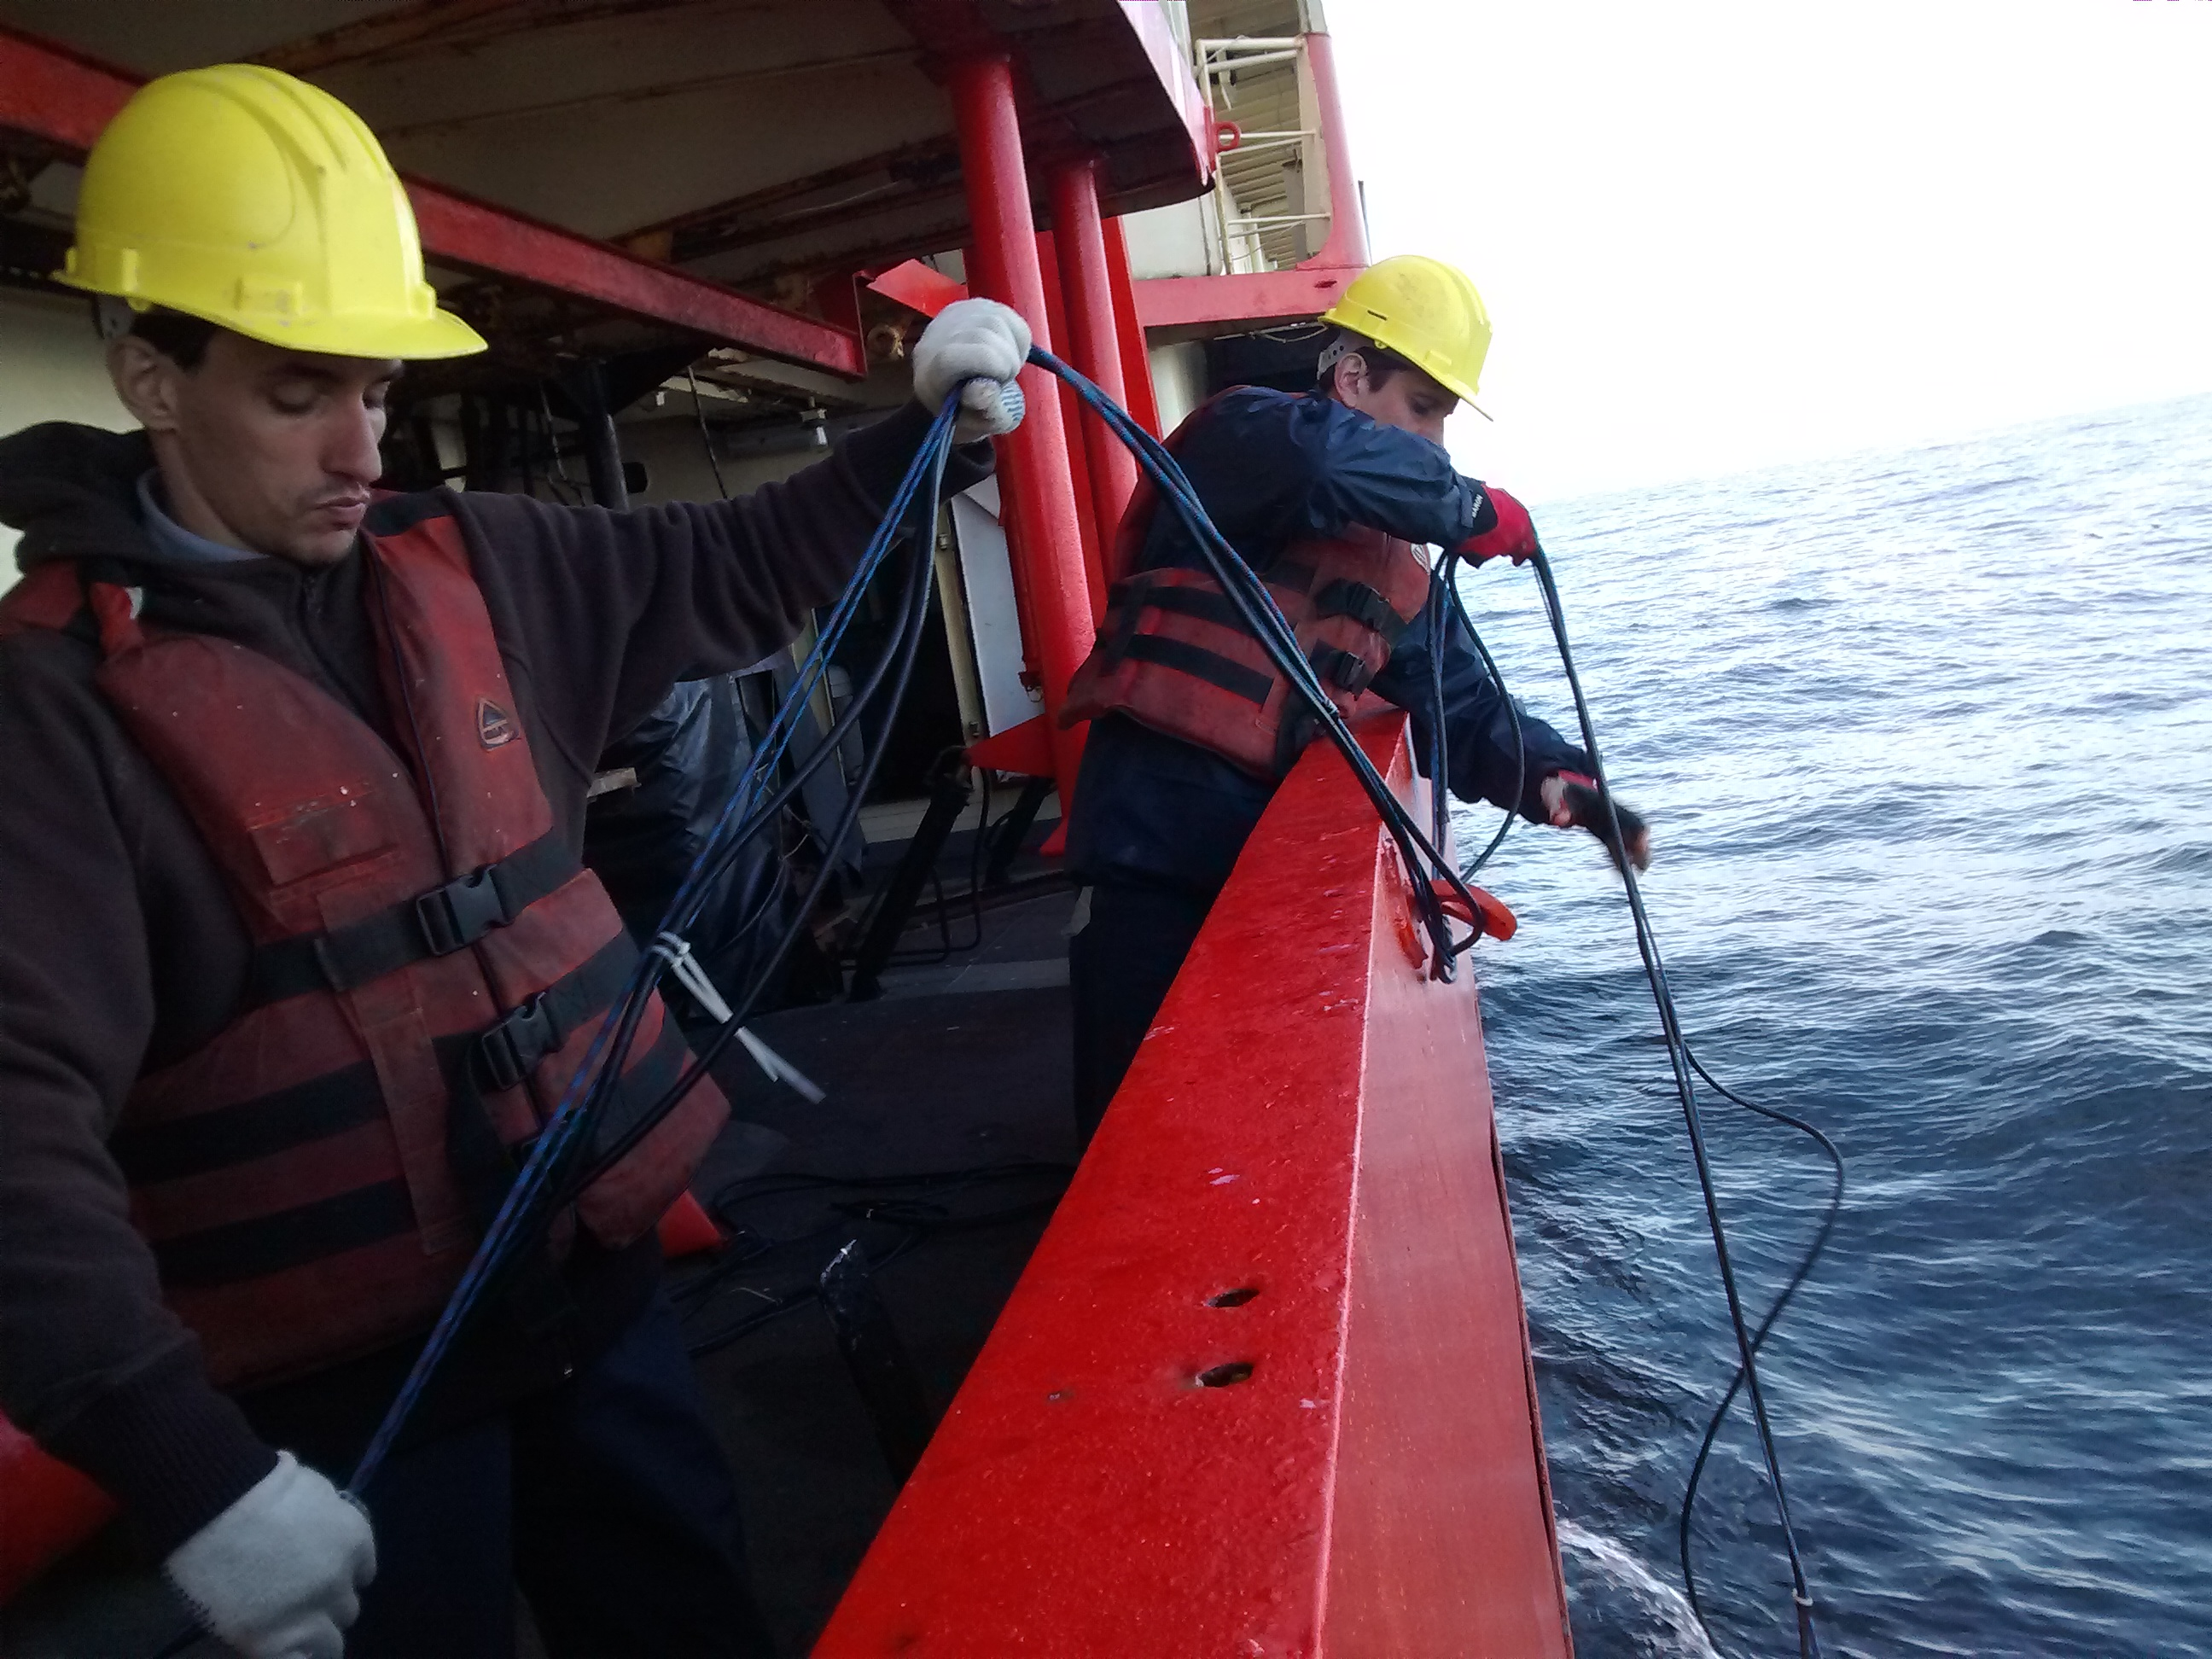
\includegraphics[width=.9\textwidth]{./imagenes/antecedentes.jpg}
\end{frame}

\begin{frame}[c]{\textbf{\LARGE{Objetivo}}}{General}
  \fontsize{18pt}{18}\selectfont
	\begin{itemize}
		\item Prototipo de estación autónoma.
		\vspace{15px}
		\item Medición de señales acústicas.
		\vspace{15px}
		\item Medición de parámetros ambientales.
		\vspace{15px}	
		\item Almacenamiento de la información.
		\vspace{15px}	
		\item Transmisión en tiempo real.
	\end{itemize}
\end{frame}

\begin{frame}{\textbf{\LARGE{Objetivo}}}{Particular}
  \fontsize{18pt}{18}\selectfont
	\vspace{-.7cm}
	\centering
	\begin{itemize}
		\item Desarrollar un firmware de control para la CIAA-NXP.
		\vspace{15px}
		\item Arquitectura multicore modular y flexible.
		\vspace{15px}
		\item Mecanismos de comunicación y sincronización.
		\vspace{15px}	
		\item Interfaz de usuario
		%\vspace{15px}	
		%\item 
	\end{itemize}
\end{frame}
%==================================================================================
%  PLANIFICACIÓN
%==================================================================================
\section{Planificación}

\begin{frame}{\textbf{\LARGE{Diagrama en bloques}}}
%	\vspace{-.6cm}
	\includegraphics<1>[width=\textwidth]{./imagenes/Diagrama_en_Bloques.pdf}
	\includegraphics<2>[width=\textwidth]{./imagenes/Diagrama_en_Bloques_recorte.pdf}
\end{frame}

\begin{frame}{\textbf{\LARGE{Planificación en etapas}}}
	\vspace{-.7cm}
	\begin{figure}[H]
		{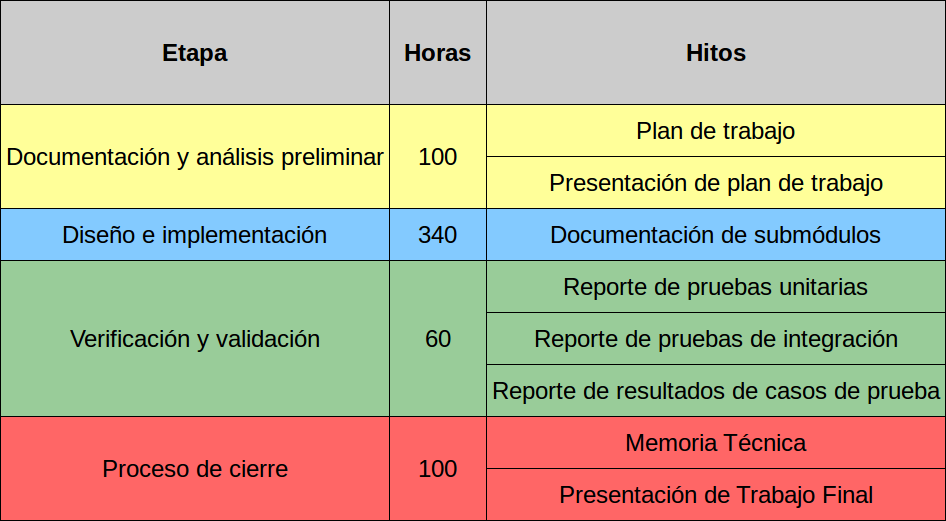
\includegraphics[width=\textwidth]{./imagenes/planificacion.png}}
	\end{figure}	
\end{frame}

\begin{frame}{\textbf{\LARGE{Desglose de tareas en AoN}}}
	\vspace{-.7cm}
	\begin{figure}[H]
		{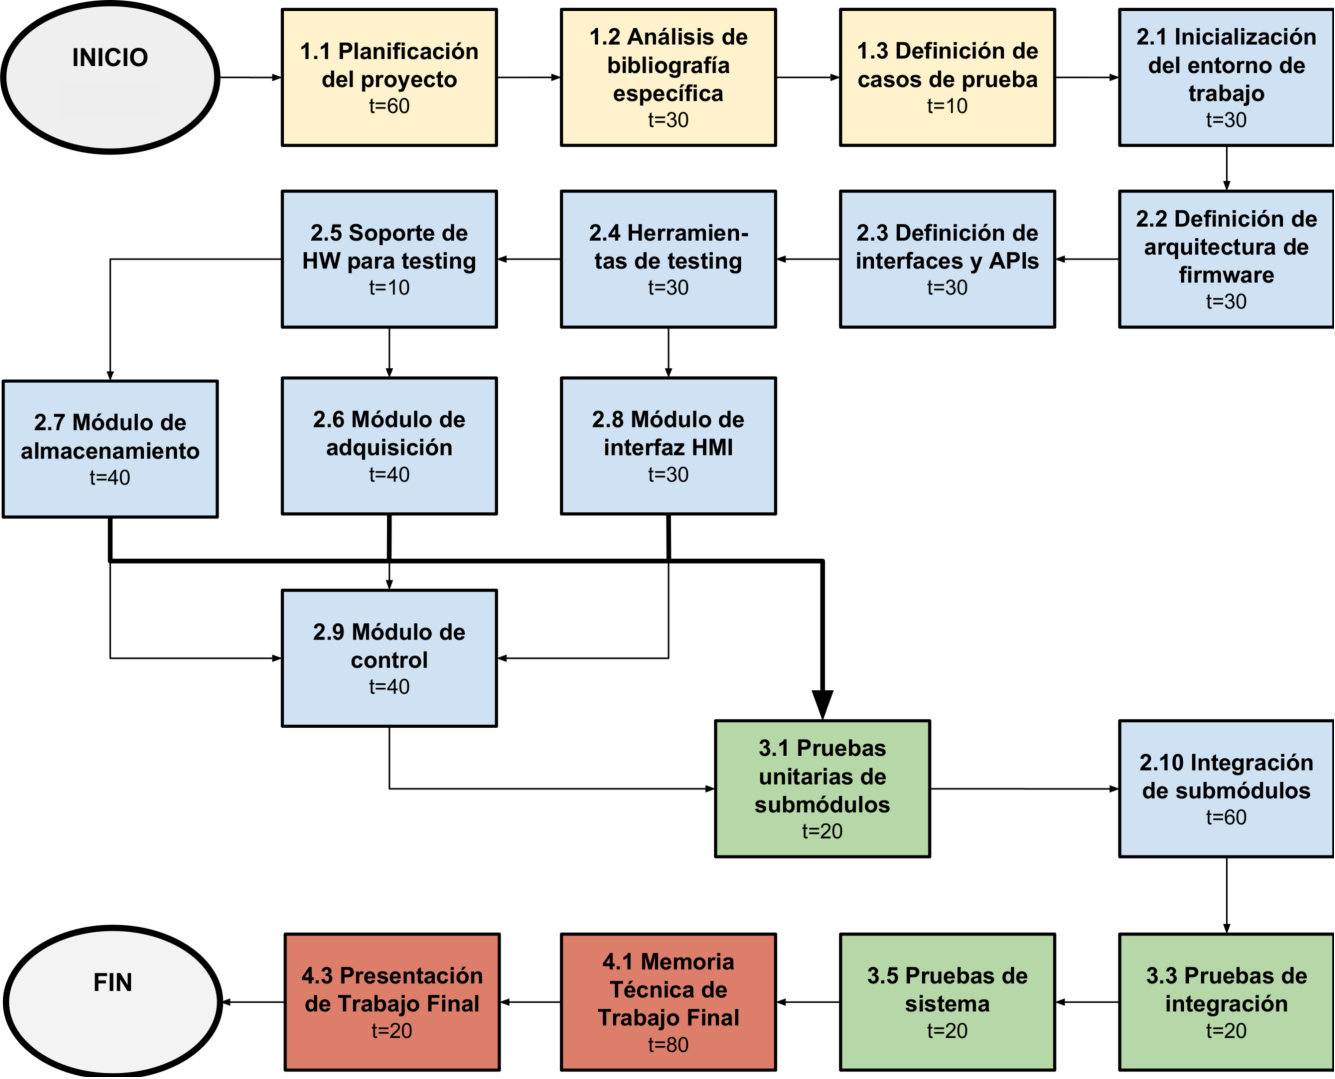
\includegraphics[height=.8\textheight]{./imagenes/AoN.pdf}}
	\end{figure}	
\end{frame}

%==================================================================================
%   METODOLOGÍA
%==================================================================================
\section{Metodología}

\begin{frame}{\textbf{\LARGE{Modelo de ramas}}}{Successfull git branch model}
	\fontsize{16pt}{16}\selectfont
	\vspace{-.9cm}
	\begin{columns}
	  \column{.5\textwidth}
%	  	\vspace{-.9cm}
	  \begin{figure}[H]
    		\includegraphics<1->[height=.8\textheight]{./imagenes/Git-branching-model.pdf}
	  \end{figure}	
	\hfill
	\column{.5\textwidth} 	
	Ramas creadas:
	\vspace{5px}
	  \begin{itemize}[]
		  \item Master
		  \item Develop
		  \item Adquisición
	  	  \item Almacenamiento
	  	  \item Interfaz de usuario
	 	  \item Control
	 	  \item Ceedling
	  \end{itemize}
	\end{columns}
\end{frame}


\begin{frame}{\textbf{\LARGE{Inter Process Communications}}}
	\vspace{-.7cm}
	\begin{figure}[H]
		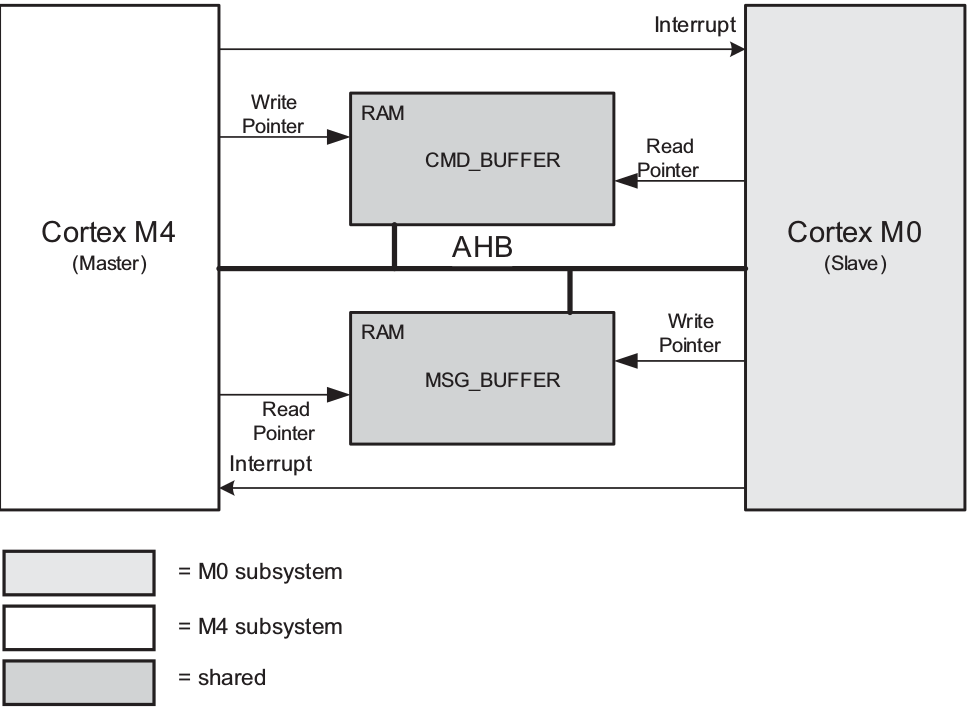
\includegraphics[height=.8\textheight]{./imagenes/IPC.png}
	\end{figure}	
\end{frame}

\begin{frame}{\textbf{\LARGE{Protothreads}}}{Multitasking cooperativo}
	\vspace{-.7cm}
	\fontsize{18pt}{18}\selectfont
	\vspace{-.7cm}
	\centering
	\begin{itemize}
		\item Abstracción computacional para multitasking cooperativo.
		\vspace{15px}
		\item Bloqueo de tareas sin cambio de contexto.
		\vspace{15px}
		\item 2 bytes de overhead por thread
		\vspace{15px}	
		\item Conjunto de macros o co-rutinas
	%	\item 
	\end{itemize}
\end{frame}
%==================================================================================
%  IMPLEMENTACIÓN
%==================================================================================
\section{Implementación}

\begin{frame}{\textbf{\LARGE{Modelo de capas}}}
	\vspace{-.7cm}
	\begin{figure}[H]
		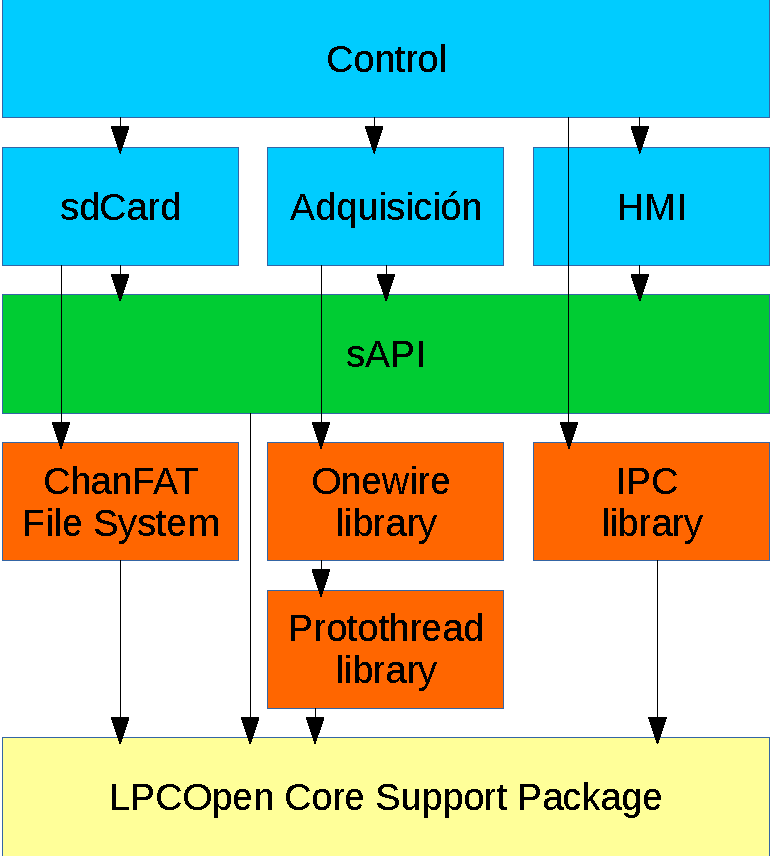
\includegraphics[height=.8\textheight]{./imagenes/capas.pdf}
	\end{figure}	
\end{frame}

\begin{frame}{\textbf{\LARGE{Máquina de Estados Finitos}}}{Módulo genérico}
	\vspace{-1.1cm}
	\begin{figure}[H]
		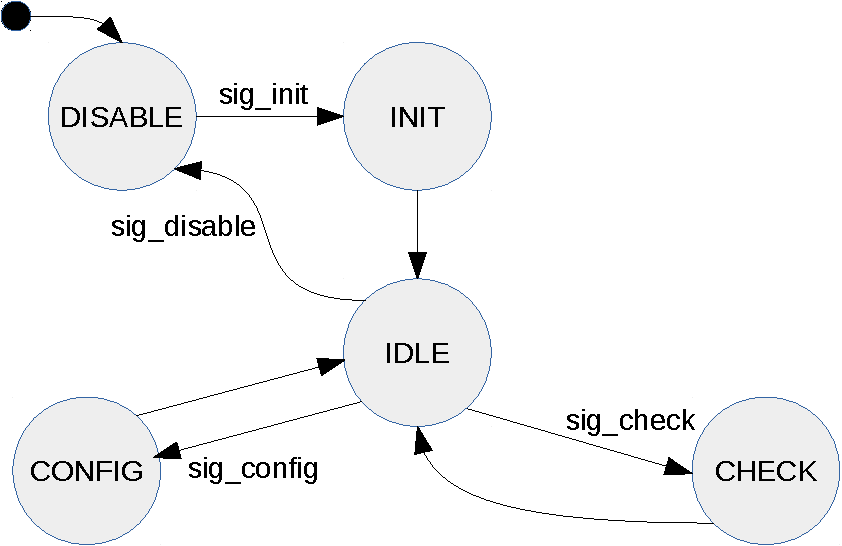
\includegraphics[height=.8\textheight]{./imagenes/MEF_generica.pdf}
	\end{figure}	
\end{frame}

\begin{frame}{\textbf{\LARGE{Máquina de Estados Finitos}}}{Módulo genérico}
	\vspace{-.7cm}
	\begin{columns}
	  \column{.45\textwidth}
	  algo
	  \column{.45\textwidth}
	  otra
	\end{columns}
\end{frame}




\begin{frame}{\textbf{\LARGE{Interfaz de usuario}}}{}
	\vspace{-.7cm}
	\centering
	\begin{figure}[H]
		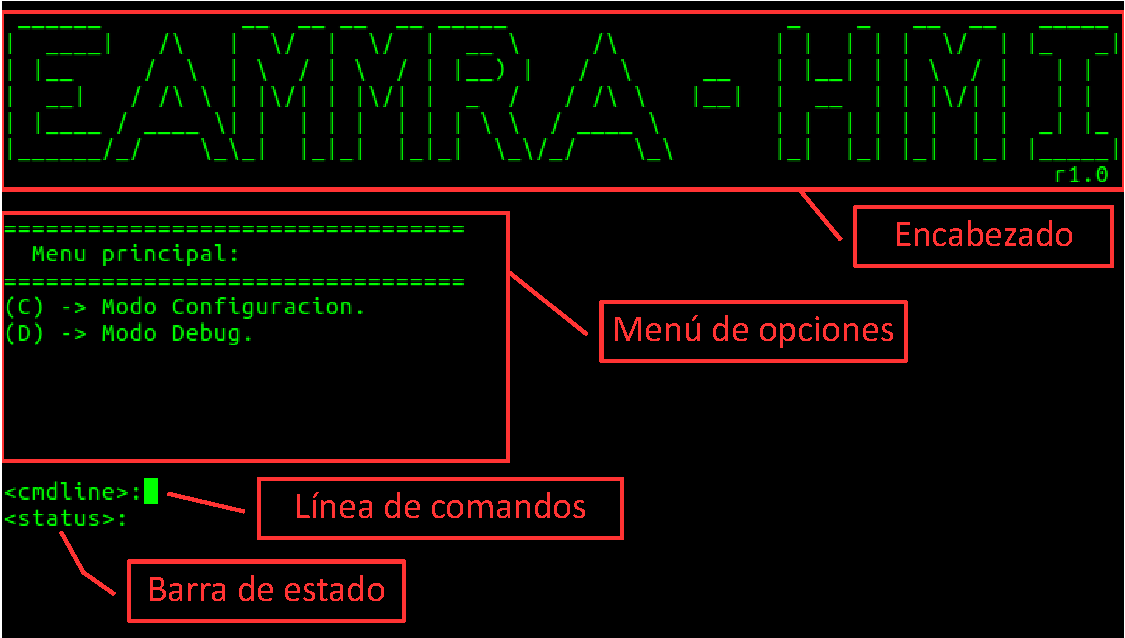
\includegraphics[width=\textwidth]{./imagenes/interfaz_detalles.pdf}
	\end{figure}	
\end{frame}


%==================================================================================
%  TESTING
%==================================================================================
\section{Testing}

\begin{frame}{\textbf{\LARGE{Modelo de ramas}}}
	\vspace{-.7cm}
	\begin{figure}[H]
		{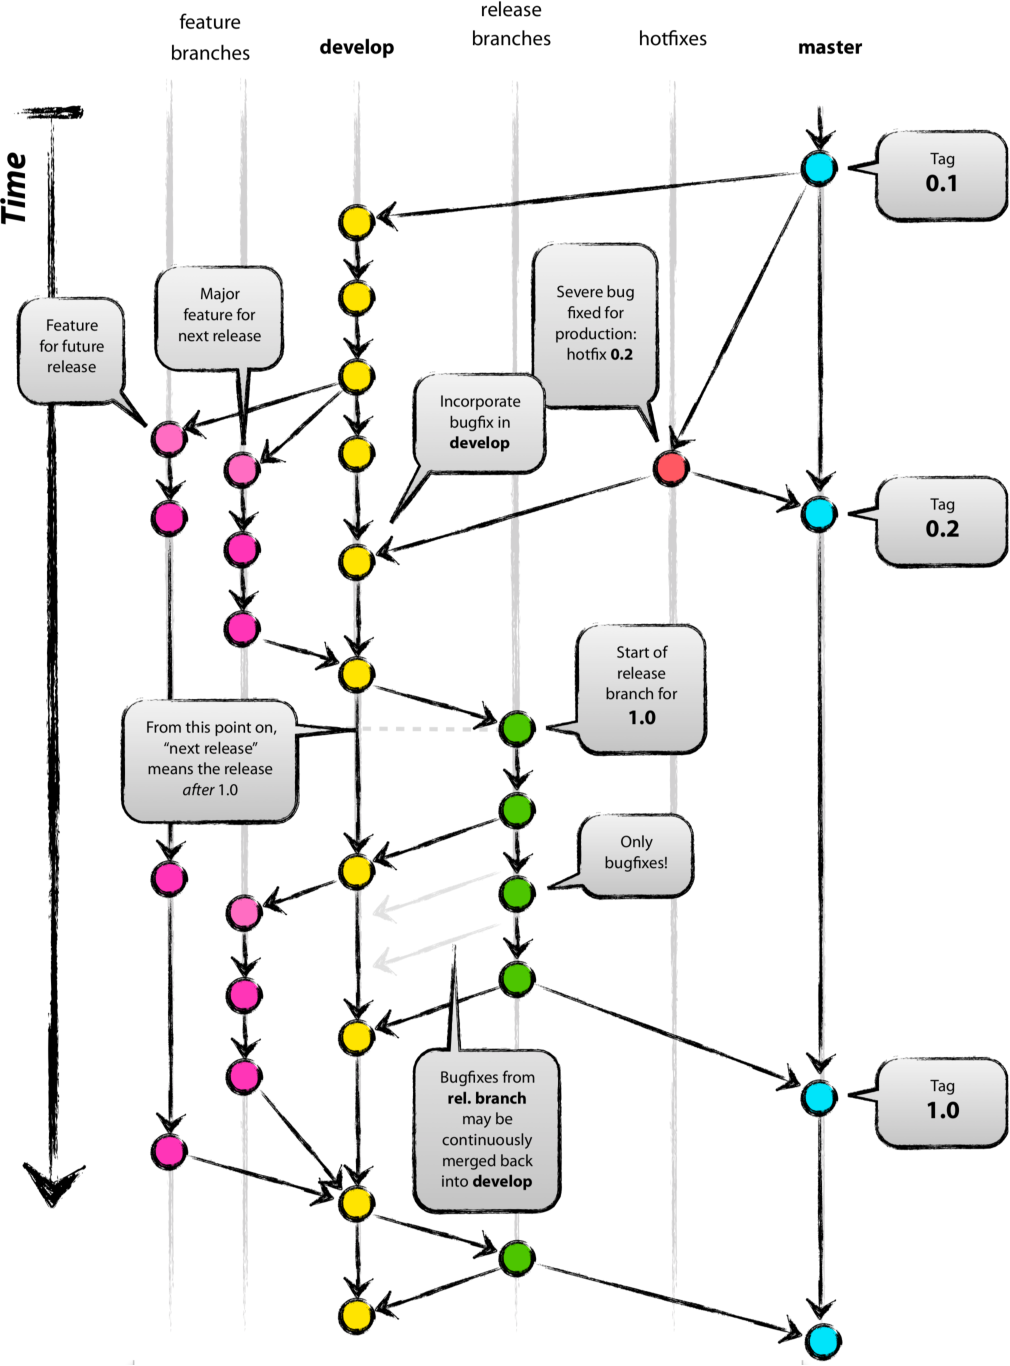
\includegraphics[height=.8\textheight]{./imagenes/Git-branching-model.pdf}}
	\end{figure}	
\end{frame}

%==================================================================================
%  DEMOSTRACIÓN
%==================================================================================
\section{Demo}

\begin{frame}{\textbf{\LARGE{Modelo de ramas}}}
	\vspace{-.7cm}
	\begin{figure}[H]
		{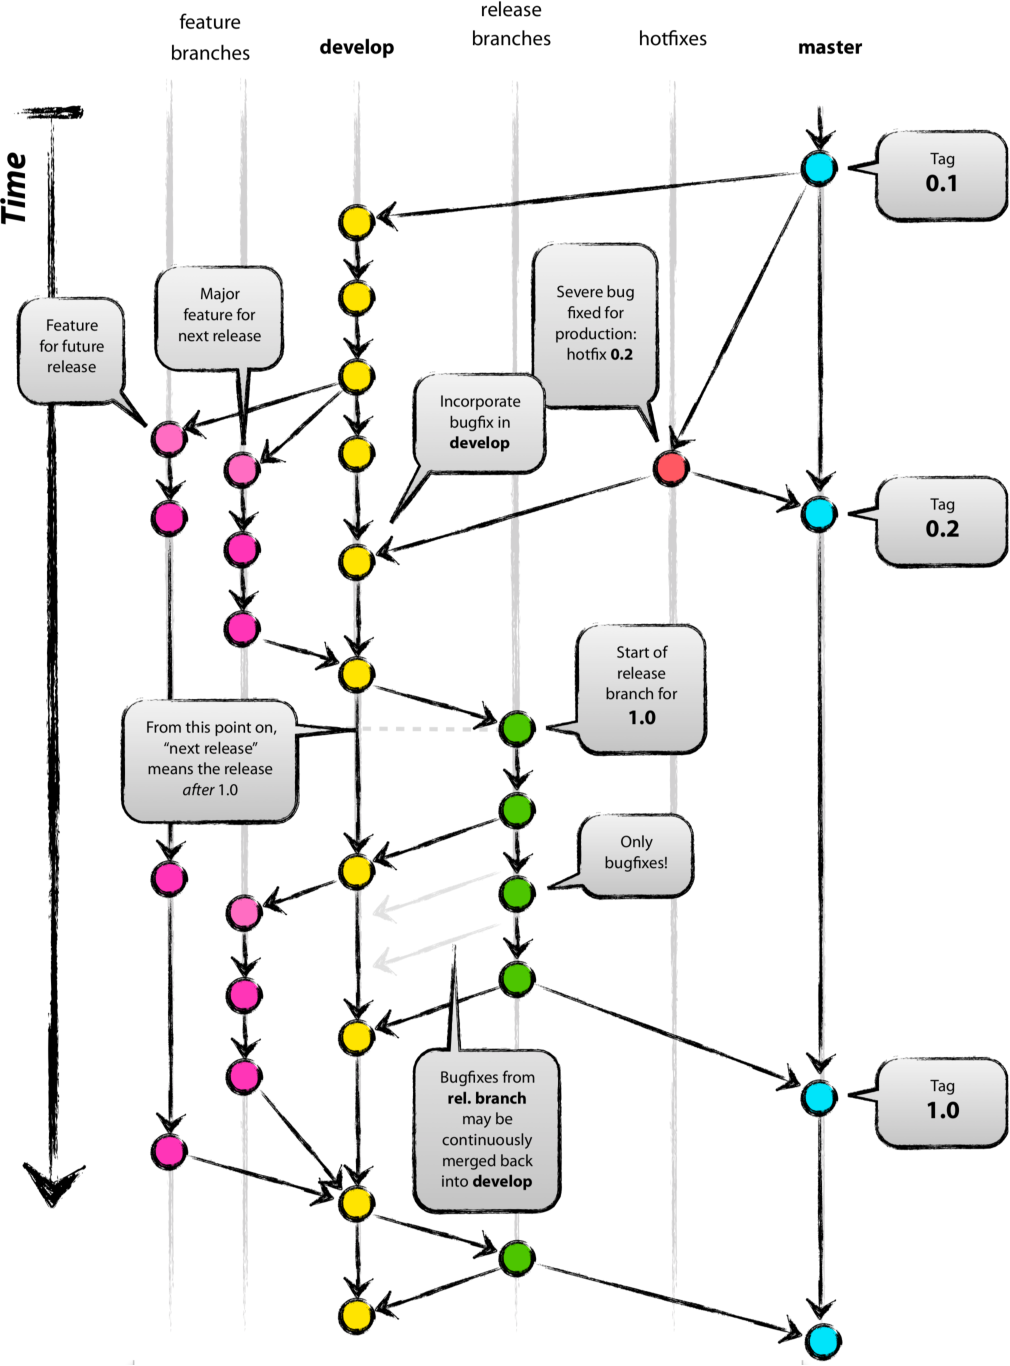
\includegraphics[height=.8\textheight]{./imagenes/Git-branching-model.pdf}}
	\end{figure}	
\end{frame}

%==================================================================================
%  CONCLUSIONES
%==================================================================================
\section{Conclusiones}



\begin{frame}{\textbf{\LARGE{¿Sobre qué hace falta alertar?}}}
\fontsize{18pt}{18}\selectfont

\end{frame}

\begin{frame}{\textbf{\LARGE{Tecnologías utilizadas}}}
\fontsize{18pt}{18}\selectfont
\end{frame}


%==================================================================================
%  PREGUNTAS
%==================================================================================
\begin{frame}[plain,c]
%\frametitle{A first slide}
\begin{center}
\usebeamerfont*{frametitle} %\usebeamercolor[fg]{frametitle}
\Huge ¿Preguntas?
\end{center}

\end{frame}


%==================================================================================
%  APÉNDICE
%==================================================================================
\begin{frame}[fragile]{\textbf{\LARGE{Protothreads}}}{Multitasking cooperativo}
	\vspace{-.7cm}
	\begin{verbatim}
		struct pt { unsigned short lc; };
		
		#define PT_THREAD(name_args)  char name_args

		#define PT_BEGIN(pt)          switch(pt->lc) { case 0:

		#define PT_WAIT_UNTIL(pt, c)  pt->lc = __LINE__; \
		                              case __LINE__: \
		                              if(!(c)) return 0

		#define PT_END(pt)            } pt->lc = 0; return 2

		#define PT_INIT(pt)           pt->lc = 0
	\end{verbatim}
\end{frame}

\begin{frame}[fragile]{\textbf{\LARGE{Protothreads}}}{Multitasking cooperativo}
	\vspace{-.6cm}
  \begin{minipage}{.5\textwidth}
    \begin{lstlisting}[frame=tlrb,basicstyle=\footnotesize,label={lst:proto1}]{Protothreads}
static
PT_THREAD(example(struct pt *pt))
{
  PT_BEGIN(pt);
  
  while(1) {
    PT_WAIT_UNTIL(pt,
      counter == 1000);
    printf("Threshold reached\n");
    counter = 0;
  }
  
  PT_END(pt);
}
    \end{lstlisting}
  \end{minipage}\hfill
  \begin{minipage}{.5\textwidth}
    \begin{lstlisting}[frame=tlrb,basicstyle=\footnotesize,label={lst:proto2}]{Traducción}
static
char example(struct pt *pt)
{
  
  switch(pt->lc) { case 0:
 
  while(1) {
    pt->lc = 12; case 12:
    if(!(counter == 1000)) return 0;
    printf("Threshold reached\n");
    counter = 0;
  }
  } pt->lc = 0; return 2;
}
    \end{lstlisting}
  \end{minipage}
\end{frame}

\end{document}
